\documentclass[a4paper, czech]{article}

\usepackage[czech]{babel}
\usepackage{indentfirst}
\usepackage{graphicx}
\usepackage{float}
\usepackage[margin=1.5cm]{geometry}
\usepackage{booktabs}
\usepackage{amsmath}
\usepackage{xcolor}
\usepackage{multirow}
\usepackage{tabularray}
\usepackage{bold-extra}

\begin{document}
\begin{table}[H]
    \centering
    \begin{tblr}{
        cell{1}{1} = {c = 2, r = 4}{c}, % Logo
        cell{1}{4} = {c = 3}{c}, % Předmět
        cell{2}{4} = {c = 3}{c}, % Jméno
        cell{3}{4} = {}{c}, % Ročník
        cell{3}{6} = {}{c}, % Studijní skupina
        cell{4}{4} = {}{c}, % Spolupracoval
        cell{4}{6} = {}{c}, % Mereno dne
        cell{5}{1} = {c = 2}{55mm}, % Kontroloval
        cell{5}{3} = {c = 2}{55mm}, % Hodnoceni
        cell{5}{5} = {c = 2}{55mm}, % Dne
        cell{6}{2} = {c = 5}{}, % Nazev ulohy
        cell{7}{1} = {}{c}, % Číslo úlohy
        cell{7}{2} = {c = 5}{c}, % Název úlohy
        vline{1,2,7} = {1.2pt},
        vline{3,5},
        hline{1,5,6,8} = {1.2pt},
        hline{2,3,4}
        }
        
\includegraphics{logo_fekt.png} & & \textsuperscript{Předmět} & \large \textbf{Měření v audiotechnice} \\
             & & \textsuperscript{Jméno} & \large \textbf{Karolína Šebestová} \\
             & & \textsuperscript{Ročník} & \large \textbf{3.} & \textsuperscript{Studijní skupina} & \large \textbf{St 14:00} \\
             & & \textsuperscript{Spolupracoval} & \large \textbf{Filip Kokavec} & \textsuperscript{Měřeno dne} & \large \textbf{30.10.2024} \\
        \textsuperscript{Kontroloval} & & \textsuperscript{Hodnocení} & & \textsuperscript{Dne} \\
        \textsuperscript{Číslo úlohy} & \textsuperscript{Název úlohy} \\
        \Large \textbf{5A AUDIO} & \Large \textsc{\textbf{Automatizované měření vlastností audio zesilovače}} \\
    \end{tblr}
\end{table}

\section{Zadání}

\begin{itemize}
    \item Pomocí programu v prostředí Keysight VEE změřte kmitočtovou charakteristiku modulu a fáze přenosu zesilovače.
    \item Pomocí osciloskopu změřte spektrum výstupního signálu ze zesilovače buzeného harmonickým signálem a vypočí- tejte hodnotu činitele harmonického zkreslení.
    \item Změřte úroveň přeslechů v zesilovači z kanálu 1 do kanálu 2.
    \item Změřte a vypočítejte úroveň odstupu signálu od šumu a rychlost přeběhu.
\end{itemize}

\section{Teoretický úvod}

\section{Výsledky měření}

\subsection{Tabulky}

\begin{table}[H]
    \catcode`\-=12
    \centering
    \caption{Automatizované měření kmitočtové charakteristiky zesilovače}
    \begin{tabular}{rcccc}
        \toprule
        \multicolumn{1}{c}{Kmitočet}   & \begin{tabular}[c]{@{}c@{}}Napětí na výstupu\\      generátoru\end{tabular} & \begin{tabular}[c]{@{}c@{}}Napětí na výstupu\\      zesilovače\end{tabular} & \begin{tabular}[c]{@{}c@{}}Modul\\      přenosu\end{tabular} & \begin{tabular}[c]{@{}c@{}}Fáze\\      přenosu\end{tabular} \\
        \cmidrule(rl){1-1}
        \cmidrule(rl){2-2}
        \cmidrule(rl){3-3}
        \cmidrule(rl){4-4}
        \cmidrule(rl){5-5}
        \multicolumn{1}{c}{$f$ {[}Hz{]}} & $U_g$ {[}V{]}                                                                  & $U_z$  {[}V{]}                    & Z {[}$\Omega${]}                                                    & $\phi$ {[}°{]}                                                   \\
        \midrule
        5          & 0,247                                                                       & 0,50                           & 6,125                                                        & -84,0                                                       \\
        7          & 0,247                                                                       & 0,56                           & 7,172                                                        & -60,4                                                       \\
        10         & 0,246                                                                       & 0,61                           & 7,845                                                        & -44,1                                                       \\
        15         & 0,246                                                                       & 0,64                           & 8,250                                                        & -29,4                                                       \\
        20         & 0,246                                                                       & 0,65                           & 8,440                                                        & -22,4                                                       \\
        30         & 0,246                                                                       & 0,66                           & 8,506                                                        & -14,6                                                       \\
        40         & 0,246                                                                       & 0,66                           & 8,572                                                        & -12,7                                                       \\
        60         & 0,246                                                                       & 0,66                           & 8,585                                                        & -6,5                                                        \\
        100        & 0,246                                                                       & 0,66                           & 8,572                                                        & -3,9                                                        \\
        200        & 0,246                                                                       & 0,66                           & 8,572                                                        & -2,8                                                        \\
        400        & 0,246                                                                       & 0,67                           & 8,703                                                        & -2,0                                                        \\
        600        & 0,246                                                                       & 0,67                           & 8,638                                                        & -1,8                                                        \\
        1 000       & 0,246                                                                       & 0,67                           & 8,703                                                        & -1,7                                                        \\
        2 000       & 0,246                                                                       & 0,67                           & 8,703                                                        & -1,0                                                        \\
        3 000       & 0,246                                                                       & 0,67                           & 8,638                                                        & -0,9                                                        \\
        4 000       & 0,246                                                                       & 0,67                           & 8,703                                                        & -1,2                                                        \\
        6 000       & 0,246                                                                       & 0,67                           & 8,638                                                        & -0,2                                                        \\
        10 000      & 0,246                                                                       & 0,67                           & 8,703                                                        & 0,9                                                         \\
        15 000      & 0,246                                                                       & 0,67                           & 8,664                                                        & 0,7                                                         \\
        20 000      & 0,246                                                                       & 0,67                           & 8,703                                                        & 2,1                                                         \\
        30 000      & 0,246                                                                       & 0,67                           & 8,729                                                        & 5,4                                                         \\
        40 000      & 0,246                                                                       & 0,64                           & 8,305                                                        & 18,2                                                        \\
        60 000      & 0,246                                                                       & 0,57                           & 7,344                                                        & 46,3                                                        \\
        100 000     & 0,245                                                                       & 0,40                           & 4,214                                                        & 80,9                                                        \\
        150 000     & 0,245                                                                       & 0,27                           & 0,747                                                        & 95,2                                                        \\
        200 000     & 0,244                                                                       & 0,20                           & -1,727                                                       & 105,5                                                       \\
        300 000     & 0,243                                                                       & 0,14                           & -5,105                                                       & 118,2                                                       \\
        400 000     & 0,242                                                                       & 0,10                           & -7,504                                                       & 147,0                                                       \\
        550 000     & 0,239                                                                       & 0,08                           & -9,615                                                       & 154,0                                                       \\
        600 000     & 0,238                                                                       & 0,08                           & -10,030                                                      & 152,0                                                       \\
        700 000     & 0,235                                                                       & 0,07                           & -10,900                                                      & -                                                           \\
        800 000     & 0,234                                                                       & 0,06                           & -11,398                                                      & -                                                           \\
        \bottomrule
    \end{tabular}
\end{table}

\subsection{Grafy}

\begin{figure}[H]
    \centering
    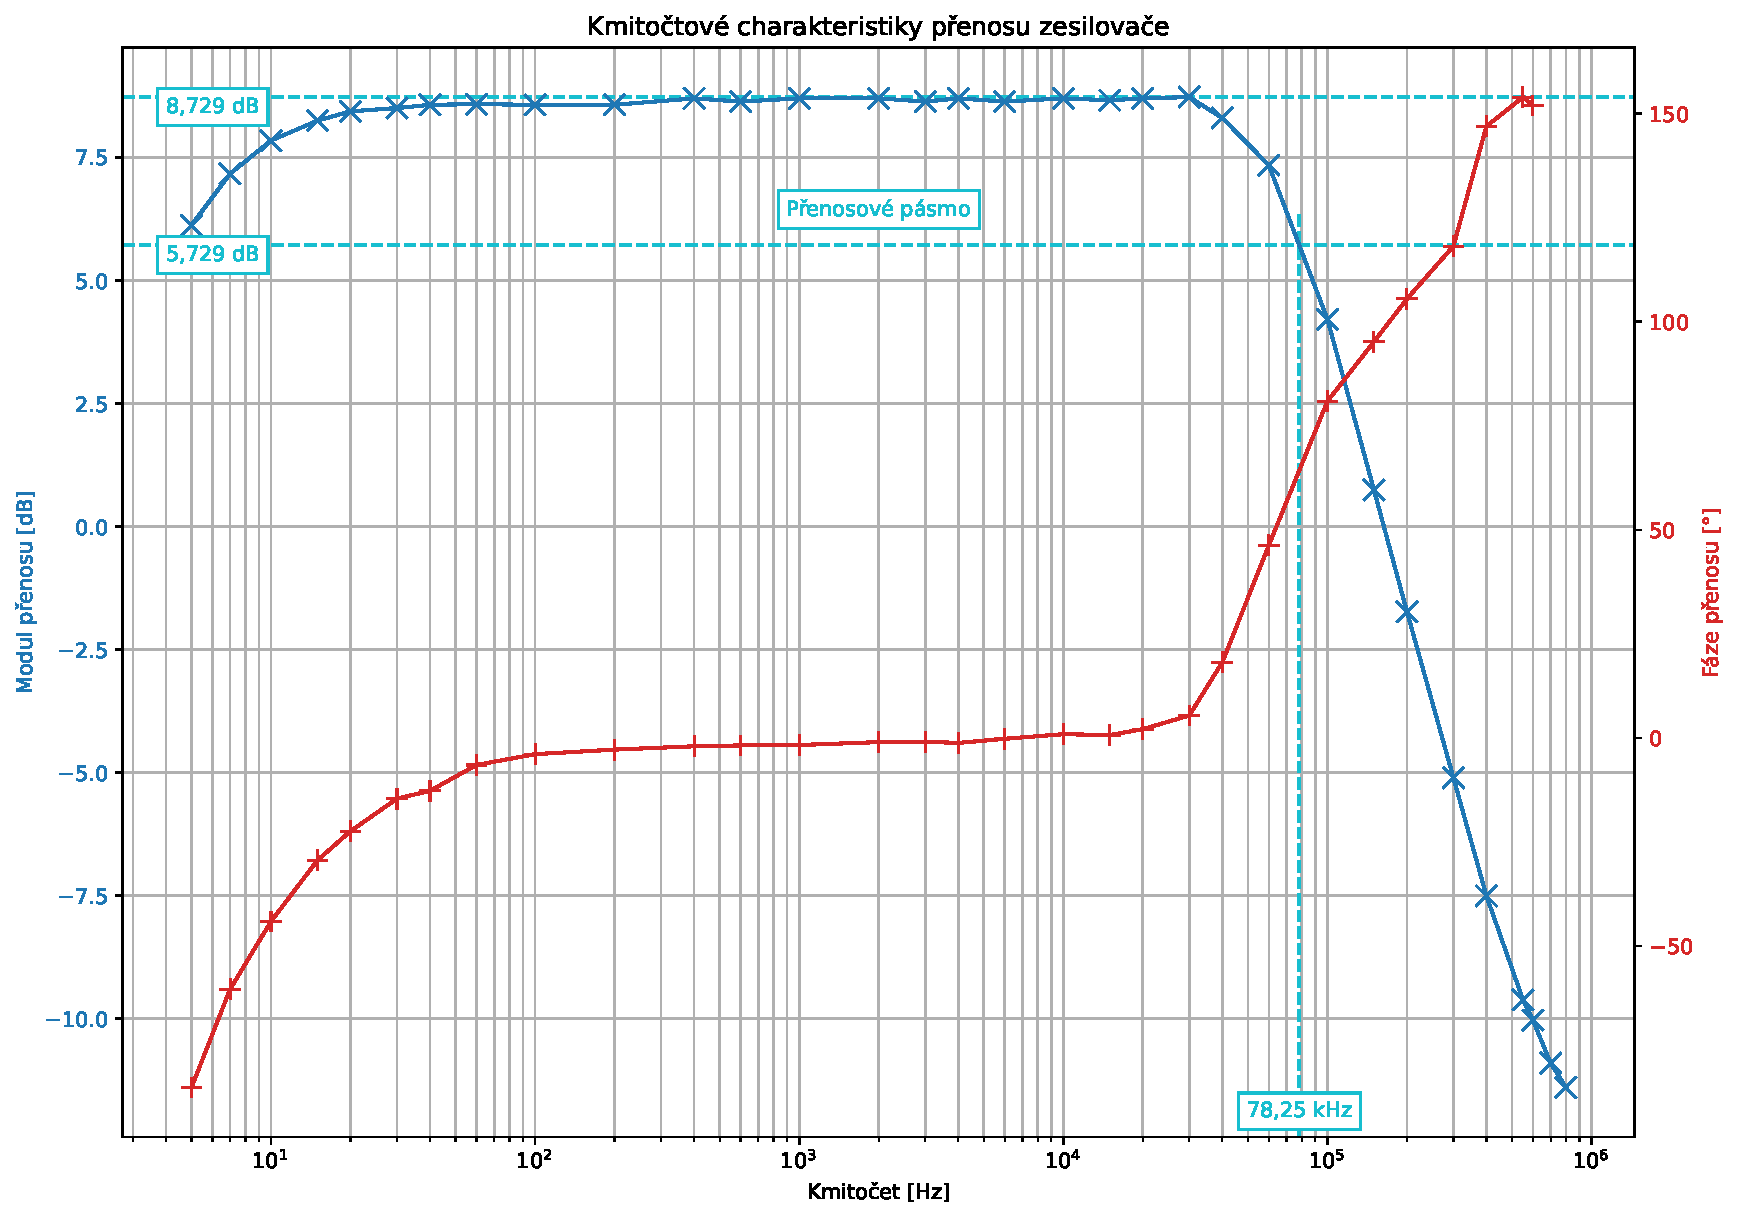
\includegraphics[width=\textwidth]{grafy/graf_kmitoctova_charakteristika.pdf}
    \caption{Kmitočtové charakteristiky přenosu zesilovače}
\end{figure}

\subsection{Příklady výpočtu}

\section{Seznam použitých přístrojů}

\section{Závěr}

\end{document}